\begin{frame}[c]{Intro} 

\begin{center}

\vspace{-0.6cm}
\begin{tikzpicture}[scale=1.1, every node/.style={scale=1.1}, node distance = 2cm, auto]
   
  \node [outer sep=0cm] (environment) at (0,0)  {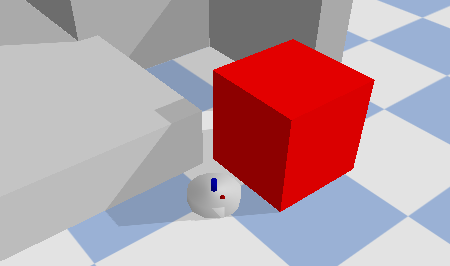
\includegraphics[width=4.6cm]{figures/introduction/example_env}};

  \draw [myEvenLighterColor,
  rounded corners=0.3cm, 
  line width=0.3cm]  
  (environment.north west) -- 
  (environment.north east) --
  (environment.south east) --
  (environment.south west) -- cycle  ;

  \node [block,
  above of=environment,
  minimum height=2cm,
  minimum width=5cm,
  node distance=4.1cm,
  outer sep=0cm] (hgraph) {Proposed Robot Framework};

  % Draw edges
  \draw[-stealth] ([yshift=0.155cm, xshift=0.4 cm]environment.north) -- node [xshift=-.05cm, right] {\shortstack[]{sensor\\measurements}}([xshift=0.4 cm]hgraph.south) ;
  \draw[-stealth] ([xshift=-0.4 cm]hgraph.south) -- node [left] {robot input}([yshift=0.155cm, xshift=-0.4 cm]environment.north) ;
  \draw[stealth-] (hgraph.west) -- node [above] {task} ++(-1, 0);

\end{tikzpicture}

\end{center}

\end{frame}
